
\section{Experiments}

\letteredsubsection{A. Datasets}

This experiment uses the ODIR-5K (Ocular Disease Intelligent Recognition)\hyperref[_Ref213949402]{{[}46{]}} dataset as the single source domain. ODIR contains 10,000 color fundus images from 5,000 patients, with one left-eye and one right-eye image for each patient. The images were initially annotated by three ophthalmologists with more than two years of clinical experience and then adjudicated by three experts with more than ten years of experience. The dataset defines eight non-mutually exclusive classes: normal (N), Diabetic Retinopathy (D), Glaucoma (G), Cataract (C), Age-related Macular Degeneration (A), Hypertension (H), Myopia (M), and Others (O), as shown in \hyperref[fig:odir-samples]{Fig.~\ref*{fig:odir-samples}.a} to \hyperref[fig:odir-samples]{Fig.~\ref*{fig:odir-samples}.h}. This setting is a typical multi-label ocular disease recognition task. Each image may have multiple disease labels, and patient-level labels are determined by combining diagnostic keywords from both eyes. The official split divides the 5,000 patients into three subsets: the training set with 3,500 patients for model training, the Off-site test set with 500 patients for model selection, and the On-site test set with 1,000 patients for evaluating in-domain generalization performance. The class distribution is shown in \hyperref[tab:dataset-distribution]{Table~\ref*{tab:dataset-distribution}}, indicating class imbalance.

% Chapter 4 Experiments - Table 1
% Label distribution across the ODIR training and test splits.
\begin{table}[!htb]
\centering
\caption{Distribution of samples in each class of the ODIR dataset across the training set, On-site test set, and Off-site test set. The normal (N), Diabetic Retinopathy (D), and Others (O) classes contain relatively more samples, whereas Hypertension (H) has the fewest samples, indicating clear class imbalance.}
\label{tab:dataset-distribution}
\resizebox{\textwidth}{!}{
\begin{tabular}{lcccccccc}
\toprule
Labels & N & D & G & C & A & H & M & O \\
\midrule
Training & 1138 & 1130 & 215 & 212 & 164 & 103 & 174 & 982 \\
On-site test & 324 & 327 & 58 & 65 & 49 & 30 & 46 & 275 \\
Off-site test & 162 & 163 & 32 & 31 & 25 & 16 & 23 & 136 \\
All & 1624 & 1620 & 305 & 308 & 238 & 149 & 243 & 1393 \\
\bottomrule
\end{tabular}
}
\end{table}


\begin{figure}[!htb]
\centering
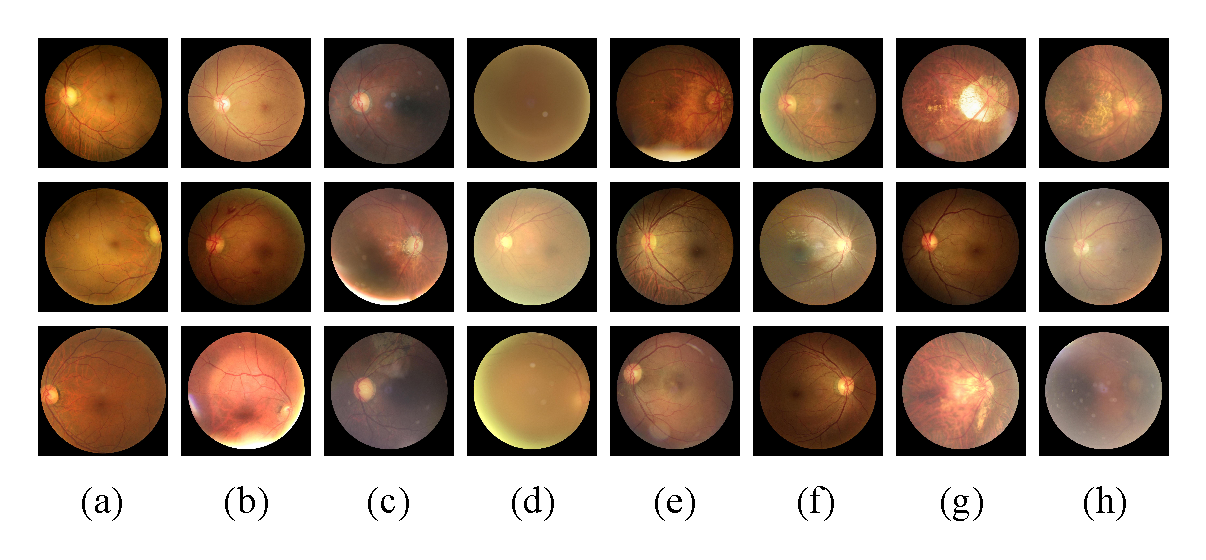
\includegraphics[width=0.86\textwidth]{./images/media/image5_padded.pdf}
\caption{Example fundus images of the eight classes in the ODIR dataset, corresponding to the eight non-mutually exclusive classes used in this study. (a)--(h) denote (a) normal (N), (b) Diabetic Retinopathy (D), (c) Glaucoma (G), (d) Cataract (C), (e) Age-related Macular Degeneration (A), (f) Hypertension (H), (g) Myopia (M), and (h) Others (O), respectively.}
\label{fig:odir-samples}
\end{figure}

To comprehensively evaluate domain generalization capability, in addition to ODIR in-domain generalization, this study introduces RFMiD\hyperref[_Ref213949409]{{[}47{]}}, provided by the RIADD challenge, as the first independent cross-domain generalization dataset. RFMiD contains 3,200 color fundus images, with 1,920, 640, and 640 images in the training, validation, and test sets, respectively. It covers 45 retinal diseases or abnormalities annotated by professional retina specialists. Some of its 45 labels overlap with the eight labels in ODIR, providing a basis for model generalization. \hyperref[fig:rfmid-samples]{Fig.~\ref*{fig:rfmid-samples}.a} to \hyperref[fig:rfmid-samples]{Fig.~\ref*{fig:rfmid-samples}.h} show representative images from eight of the 45 categories. Since the complete label spaces of RFMiD and ODIR are inconsistent, this study selects their shared classes, Diabetic Retinopathy (D), Age-related Macular Degeneration (A), and Myopia (M), for cross-domain generalization. Under this setting, 1,907 D/A/M training images are constructed on the ODIR side, with 1,425, 255, and 253 labels for D, A, and M, respectively. On the RFMiD side, 119 validation images from these three classes are used for testing, with 83, 24, and 21 labels for D, A, and M, respectively.

\begin{figure}[!htb]
\centering
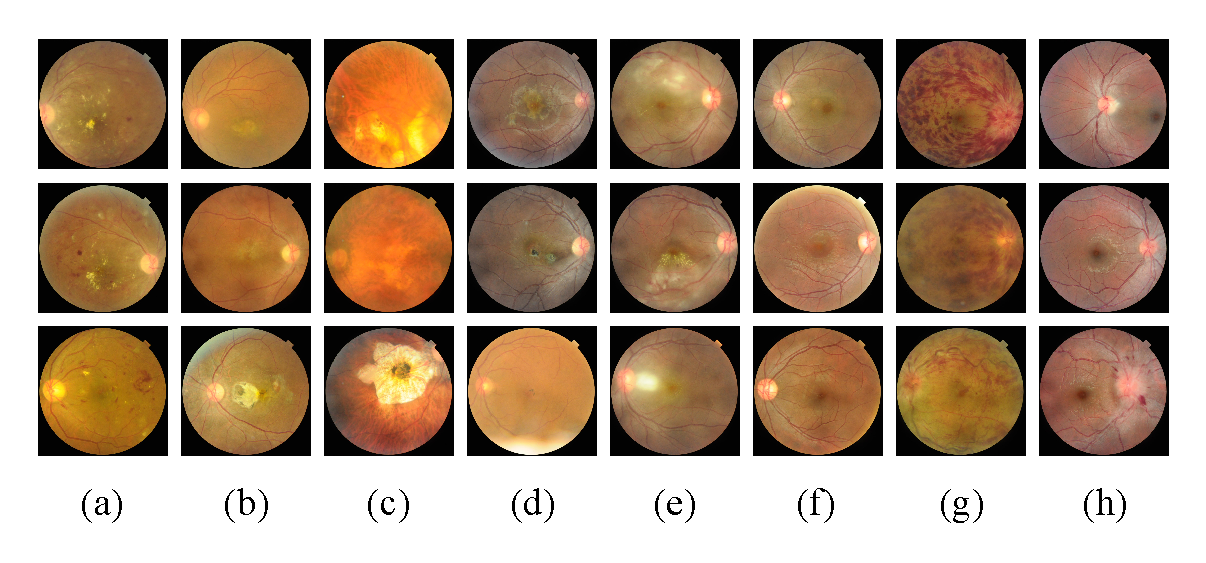
\includegraphics[width=0.86\textwidth]{./images/media/image6_padded.pdf}
\caption{Examples of eight selected fundus image classes in the RFMiD dataset. (a)--(h) correspond to (a) Diabetic Retinopathy (D), (b) Age-related Macular Degeneration (A), (c) Myopia (M), (d) Macular Scar (MS), (e) Retinitis (RS), (f) Central Serous retinopathy (CSR), (g) Central Retinal Vein Occlusion (CRVO), and (h) Disc Edema (DE), respectively. RFMiD is used as a cross-domain generalization dataset. In the experiments, the shared label space aligned with ODIR consists of D/A/M classes and is used to evaluate cross-domain generalization performance.}
\label{fig:rfmid-samples}
\end{figure}

In addition, this study introduces the EDID\hyperref[_RefEDID2024]{{[}48{]}} dataset collected from Anawara Hamida and B.N.S.B. Zahurul Haque Eye Hospital as the second independent cross-domain generalization dataset, further validating the generalization performance of the proposed method across different data sources and label organizations. The original EDID dataset contains 5,335 fundus images covering 10 single-label classes, including Central Serous retinopathy, Diabetic Retinopathy, Disc Edema, Glaucoma, normal, Macular Scar, Myopia, Pterygium, Retinal Detachment, and Retinitis Pigmentosa, with 101, 1,509, 127, 1,349, 1,024, 444, 500, 17, 125, and 139 samples, respectively. \hyperref[fig:edid-samples]{Fig.~\ref*{fig:edid-samples}.a} to \hyperref[fig:edid-samples]{Fig.~\ref*{fig:edid-samples}.h} show examples of eight representative fundus image classes selected from EDID.

\begin{figure}[!htb]
\centering
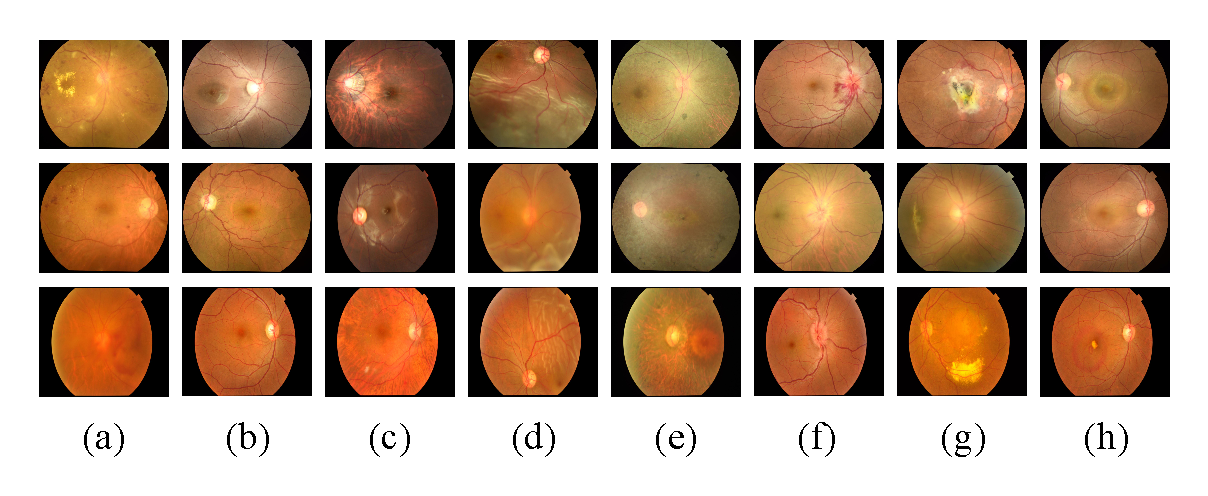
\includegraphics[width=0.86\textwidth]{./images/media/edid_samples_padded.pdf}
\caption{Examples of eight selected fundus image classes in the EDID dataset. (a)--(h) correspond to (a) Diabetic Retinopathy (D), (b) Glaucoma (G), (c) Myopia (M), (d) Retinal Detachment (RD), (e) Retinitis Pigmentosa (RP), (f) Disc Edema (DE), (g) Macular Scar (MS), and (h) Central Serous retinopathy (CSR), respectively. EDID is used as a single-label cross-domain generalization dataset. In the experiments, the shared label space aligned with ODIR consists of D/G/M classes and is used to evaluate generalization performance under different data sources and label organizations.}
\label{fig:edid-samples}
\end{figure}

Similar to RFMiD, since the complete label spaces of EDID and ODIR are inconsistent, this study selects their shared classes, Diabetic Retinopathy (D), Glaucoma (G), and Myopia (M), to construct a cross-domain generalization dataset with 3,358 images, including 1,509, 1,349, and 500 samples for D, G, and M, respectively. Since EDID is a single-label dataset, it is treated as a special case of the multi-label recognition task, where each image has only one positive label, and cross-domain generalization is evaluated in the D/G/M three-class space. Correspondingly, a D/G/M training subset is constructed on the ODIR side, containing 1,871 images, with 1,401, 227, and 243 samples for D, G, and M, respectively.

\letteredsubsection{B. Experimental Settings}

All experiments use ResNet50 as the backbone and are implemented in PyTorch. The evaluation metrics follow the official ODIR standard: Kappa, F1, AUC, and their average value, Final score. The Kappa threshold is fixed at 0.5, and F1 uses micro averaging to alleviate the influence of class imbalance.

For the baseline, we follow the original ResNet50 implementation of ODIR and modify it for our setting. The original paper uses paired binocular samples as input, evaluates different feature-level fusion strategies such as concat, prod, and sum, and then uses eight independent classification heads for patient-level prediction. In contrast, we use monocular images as input samples, with each sample carrying its corresponding patient identifier. The classifier is implemented as a single multi-label classification head, which outputs eight-dimensional logits and obtains disease probabilities through Sigmoid activation. The loss function is standard binary cross entropy (BCE). During inference, monocular predictions from the left and right eyes of the same patient are logically merged to obtain patient-level predictions, fully aligning with the official metrics. This modification avoids noise amplification caused by feature fusion and dilution of individual-difference information, and is especially advantageous when disease severity differs between the two eyes.

The training configuration is as follows. Adam is used as the optimizer, with an initial learning rate of \(1 \times 10^{-5}\). OneCycleLR is adopted as the scheduling strategy: the learning rate linearly warms up to the peak value of \(1 \times 10^{-5}\) during the first 10\% of epochs and then anneals during the remaining 90\% of epochs to facilitate convergence. The number of training epochs is 50, the batch size is 32, and the input resolution is \(448 \times 448\). The proposed method is trained on two RTX 4080 Super GPUs. Experimental results show that our improved baseline model, with an Off-site binocular Final score of 76.19, outperforms the ResNet50 implementation in the original ODIR paper, which reports an Off-site binocular Final score of 68.00.

\letteredsubsection{C. Comparison with Existing Methods}

To evaluate the recognition performance of the proposed method on the ODIR dataset, we select four representative multi-label ocular disease recognition methods, including the official baseline provided in the ODIR dataset paper by Li et al.\hyperref[_Ref213949402]{{[}46{]}} and three subsequent works by Gour and Khanna\hyperref[_Ref214903299]{{[}49{]}}, He et al.\hyperref[_Ref213950338]{{[}20{]}}, and Ou et al.\hyperref[_Ref214903327]{{[}50{]}}. These methods mainly focus on improving Final score and do not consider cross-domain generalization or privacy preservation.

Gour and Khanna\hyperref[_Ref214903299]{{[}49{]}} proposed a transfer-learning-based CNN framework with VGG16 as the backbone. The ODIR dataset is expanded through data augmentation, and the model is fine-tuned using the SGD optimizer. The method uses pretrained weights to capture structural abnormalities involving vessels, optic discs, and maculae, thereby improving recognition performance in multi-class co-occurrence scenarios.

He et al.\hyperref[_Ref213950338]{{[}20{]}} developed a dense correlation network (DCNet), which includes a backbone CNN for extracting binocular features, a spatial correlation module for capturing pixel-level relevance, and a classifier for generating patient-level classification results. Its core idea is to fuse binocular features through dense convolutional blocks and model disease co-occurrence such as DR and AMD, but it relies on binocular input.

Ou et al.\hyperref[_Ref214903327]{{[}50{]}} designed a two-stream interactive CNN. A feature enhancement module captures local-global binocular dependencies through an attention mechanism, and a multi-scale module aggregates features at different resolutions to enrich representations. The method enhances lesion regions, such as microaneurysms and hemorrhages, through two-stream interaction to improve multi-label recognition performance, but it does not consider privacy or cross-domain scenarios.

\hyperref[tab:sota-compare]{Table~\ref*{tab:sota-compare}} compares binocular metrics on the Off-site test and On-site test sets. The proposed method achieves a Final score of 78.85 on Off-site, outperforming BFENet [50] by 0.85, and achieves 77.49 on On-site, outperforming BFENet [50] by 0.79. These results demonstrate the effectiveness of dual-branch guided feature learning and adaptive label-feature relevance construction on the ODIR multi-label recognition task.

\input{manuscripts/trans/tables/src/table7_sota_trans.tex}

Existing comparison methods mainly optimize internal multi-label recognition metrics on ODIR and rarely consider domain generalization and privacy preservation simultaneously. In contrast, in addition to achieving higher Final scores on ODIR Off-site and On-site, this study validates unseen-domain performance on two cross-domain generalization datasets, RFMiD and EDID, and further evaluates performance degradation under privacy-preserving training. These results indicate that the proposed method is not limited to improving recognition performance on a single dataset, but is also designed for clinically relevant settings where data sharing is restricted and privacy preservation is required.

\letteredsubsection{D. Ablation Study Results}

To assess the independent contributions and synergistic gains of the two core modules in the proposed method, namely Dual-Branch Guided Domain-Invariant Feature Extraction (DFE) and Adaptive Label-Feature Relevance Construction (ARC), and to examine the improvement in model interpretability brought by CAM guidance, we conduct module-wise ablation experiments using ODIR Off-site binocular metrics. The results are shown in \hyperref[tab:ablation]{Table~\ref*{tab:ablation}}.

% Chapter 4 Experiments - Table 3
% Ablation study of DFE and ARC modules.
\begin{table}[!htb]
\centering
\caption{Ablation study results. The table reports binocular metrics on the ODIR Off-site test set. Compared with ResNet50 (baseline), DFE and ARC improve Final score by 2.18 and 0.79, respectively. Combining the two modules further increases the overall gain to 2.66 and achieves the best results on all four metrics, indicating positive synergy between the two modules.}
\label{tab:ablation}
\begin{tabular}{lcccc}
\toprule
Model & Kappa & F1 & AUC & Final \\
\midrule
ResNet50 & 52.75 & 87.83 & 88.00 & 76.19 \\
ResNet50+DFE & 56.20 & 88.80 & 90.10 & 78.37 \\
ResNet50+ARC & 53.19 & 87.45 & 90.29 & 76.98 \\
\textbf{ResNet50+DFE+ARC (Ours)} & \textbf{57.05} & \textbf{89.03} & \textbf{90.48} & \textbf{78.85} \\
\bottomrule
\end{tabular}
\end{table}


\begin{itemize}
\item

  ResNet50: only a single-branch ResNet50 and a standard multi-label classification head are used. The Final score is 76.19, Kappa is 52.75, and AUC is 88.00.
\item

  ResNet50+DFE: only the complete Dual-Branch Guided Domain-Invariant Feature Extraction module is introduced. The Final score increases to 78.37 (+2.18), Kappa increases by 3.45, and AUC increases by 2.10. The improvement mainly comes from CAM-guided residual weighting and the mask mechanism, which effectively suppress domain-specific noise and encourage the model to focus on domain-invariant features.

\item

  ResNet50+ARC: only the Adaptive Label-Feature Relevance Construction module is introduced. The Final score increases to 76.98 (+0.78), Kappa increases by 0.44, and AUC increases by 2.29. By explicitly modeling disease co-occurrence dependencies, such as DR and AMD or Myopia and optic-disc abnormalities, this module reduces the false-negative rate and improves multi-label recognition performance.
\item

  ResNet50+DFE+ARC (the proposed method, ours): when both modules are enabled, the Final score further increases to 78.85 (+2.66 over the baseline), Kappa reaches 57.05 (+4.30), and F1 and AUC reach 89.03 (+1.20) and 90.48 (+2.48), respectively. The total gain is close to the sum of the gains from the two modules (\(2.66 < 2.18 + 0.78 = 2.96\)), suggesting positive synergy between them. DFE provides more stable domain-invariant features for ARC, enabling Transformer to learn label-label relevance and label-feature relevance more accurately. Conversely, the attention consistency loss of ARC further constrains the output distributions of the two branches and improves feature stability. In addition, the visualization results in \hyperref[fig:cam-visualization]{Fig.~\ref*{fig:cam-visualization}} show that, compared with the baseline, the CAMs obtained by the proposed method respond less to image edges and illumination artifacts, and the model-attended regions concentrate more on the eyeball, vessels, and other disease-related regions, indicating enhanced model interpretability.
\end{itemize}

\begin{figure}[!htb]
\centering
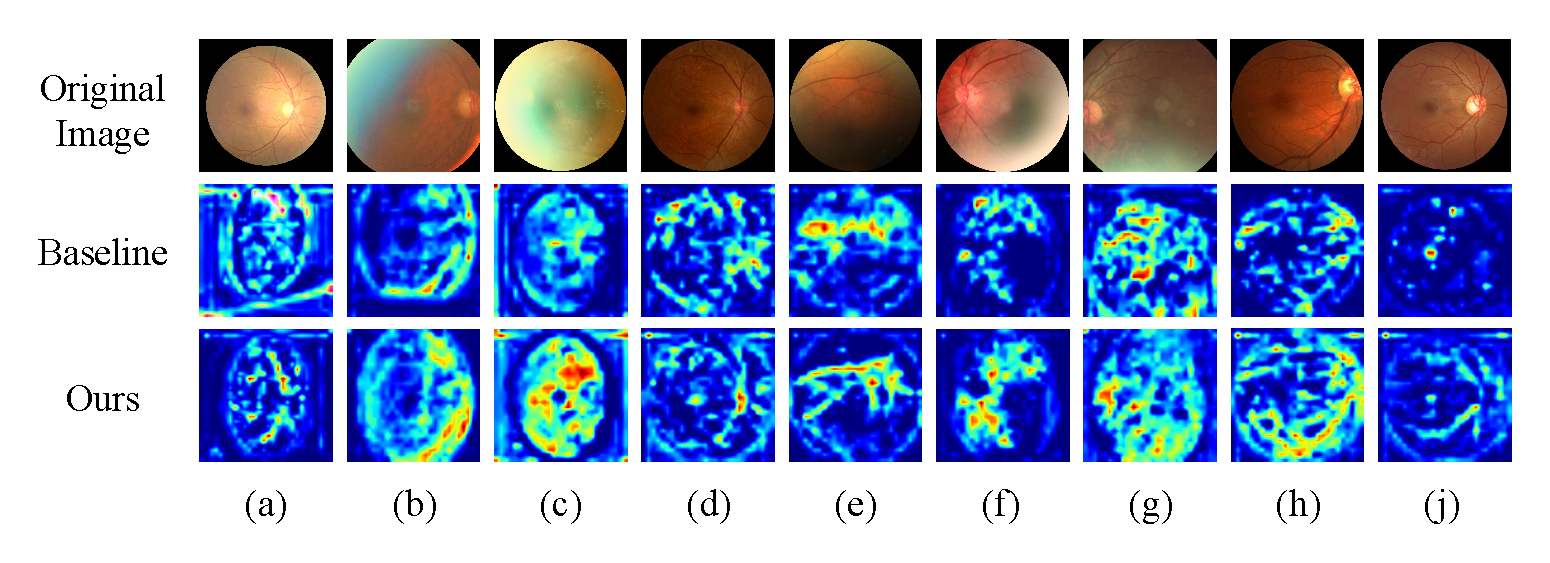
\includegraphics[width=0.92\textwidth]{./images/media/image8_padded.pdf}
\caption{Comparison of CAM-based model-attended region visualizations between the baseline and the proposed method on selected ODIR Off-site samples, where (a)--(j) denote different test samples. Compared with the baseline, the model-attended regions of the proposed method are more concentrated on the eyeball, vessels, and disease-related regions, with weaker responses to irrelevant background factors such as image edges and illumination artifacts. This indicates that the proposed method effectively suppresses domain-specific noise and enhances interpretability.}
\label{fig:cam-visualization}
\end{figure}

The ablation results show that Adaptive Label-Feature Relevance Construction (ARC) improves label relevance modeling in multi-disease co-occurrence scenarios, while Dual-Branch Guided Domain-Invariant Feature Extraction (DFE) supports learning domain-invariant features from a single source domain when multi-institutional joint training is restricted. The integration of the two modules further improves multi-label recognition performance under single-source-domain training and provides a basis for the subsequent cross-domain generalization results.

\letteredsubsection{E. Generalization Performance Results}

To comprehensively validate the generalization capability of the proposed method under single-source-domain training and the effectiveness of the privacy-preserving mechanism, we conduct systematic evaluations under both non-private and privacy-preserving scenarios, covering ODIR in-domain generalization (Off-site and On-site) and cross-domain generalization (RFMiD and EDID).

(1) Generalization performance under the non-private setting. The results are shown in \hyperref[tab:generalization]{Table~\ref*{tab:generalization}}, which reports the Final scores of the baseline and the proposed method on different test sets. The generalization experiments are organized along three evaluation directions: ODIR in-domain Off-site \(\rightarrow\) On-site, cross-domain generalization from ODIR to RFMiD, and cross-domain generalization from ODIR to EDID. For each direction, model selection and evaluation are based on the top five candidate checkpoints saved during training. Specifically, the checkpoint group with the best test-set performance is selected from the candidate checkpoints of the baseline and the proposed method, respectively, and the results of this checkpoint group on the source-domain Off-site set and the target domain are reported simultaneously.

% Chapter 4 Experiments - Table 4
% Generalization performance on ODIR, RFMiD/RIADD, and EDID.
\begin{table}[!htb]
\centering
\caption{Comparison of generalization performance on different test sets. The table compares the baseline and the proposed method on ODIR in-domain generalization (Off-site $\rightarrow$ On-site) and cross-domain generalization from ODIR to RFMiD and EDID, using Final score as the metric. Off-site $\rightarrow$ On-site reports both monocular and binocular results, while cross-domain generalization reports monocular results after aligning each dataset to a three-class label space. For each direction, the checkpoint with the best test-set performance is selected from candidate checkpoints. Overall, the proposed method outperforms the baseline in all evaluation directions.}
\label{tab:generalization}
\resizebox{\textwidth}{!}{
\begin{tabular}{lcccccccc}
\toprule
\multirow{3}{*}{Model} & \multicolumn{4}{c}{Off-site $\rightarrow$ On-site} & \multicolumn{2}{c}{Off-site $\rightarrow$ RFMiD} & \multicolumn{2}{c}{Off-site $\rightarrow$ EDID} \\
\cmidrule(lr){2-5}\cmidrule(lr){6-7}\cmidrule(lr){8-9}
& \multicolumn{2}{c}{Off-site} & \multicolumn{2}{c}{On-site} & Off-site & RFMiD & Off-site & EDID \\
\cmidrule(lr){2-3}\cmidrule(lr){4-5}\cmidrule(lr){6-7}\cmidrule(lr){8-9}
& Monocular & Binocular & Monocular & Binocular & Monocular & Monocular & Monocular & Monocular \\
\midrule
ResNet50 & 79.37 & 76.19 & 77.30 & 75.23 & 94.39 & 83.86 & 94.30 & 52.16 \\
\textbf{Ours} & \textbf{81.71} & \textbf{78.79} & \textbf{78.98} & \textbf{77.49} & \textbf{95.94} & \textbf{85.06} & \textbf{96.03} & \textbf{55.35} \\
\bottomrule
\end{tabular}
}
\end{table}


For ODIR in-domain generalization, the test set is On-site, and \hyperref[tab:generalization]{Table~\ref*{tab:generalization}} reports both monocular and binocular evaluation protocols. The baseline checkpoint achieves binocular scores of 76.19 and 75.23 on Off-site and On-site, respectively, whereas the corresponding checkpoint of the proposed method improves these scores to 78.79 and 77.49, with gains of 2.60 and 2.26 percentage points. The monocular metrics also increase from 79.37 and 77.30 to 81.71 and 78.98. This indicates that dual-branch guided feature learning and CAM-guided attention can enhance the model's focus on disease-related regions. Binocular metrics are lower than monocular metrics because the model is trained with monocular data. During inference, when the left-eye and right-eye predictions of the same patient are merged, an incorrect prediction from either eye may affect patient-level judgment, amplifying the effect of small monocular errors on the final metric.

For cross-domain generalization, the complete label spaces of RFMiD, EDID, and ODIR are inconsistent. Therefore, this study first reconstructs shared three-class label spaces before generalization evaluation. RFMiD is aligned using D/A/M classes, while EDID is aligned using D/G/M classes. Although EDID is a single-label dataset, it can still be used as a cross-domain generalization dataset under the three-class shared label space. Considering that the cross-domain generalization datasets differ more significantly from ODIR in imaging devices, acquisition procedures, illumination conditions, disease composition, and label definitions, model selection and evaluation are also based on the top five candidate checkpoints. The monocular Final scores of the selected checkpoint group on the three-class ODIR Off-site set and the cross-domain generalization dataset are reported simultaneously.

In RFMiD D/A/M cross-domain generalization, the baseline checkpoint obtains a Final score of 94.39 on ODIR Off-site and 83.86 on the target domain. The corresponding checkpoint of the proposed method obtains a Final score of 95.94 on ODIR Off-site and 85.06 on the target domain, improving by 1.55 and 1.20 percentage points, respectively. Detailed metrics show that the Kappa, F1, and AUC of the proposed method on RFMiD are 73.95, 87.96, and 93.27, all higher than the baseline values of 72.08, 87.11, and 92.39. In EDID D/G/M cross-domain generalization, the baseline checkpoint obtains a Final score of 94.30 on ODIR Off-site and 52.16 on the target domain. The proposed method obtains 96.03 on ODIR Off-site and 55.35 on the target domain, improving by 1.73 and 3.19 percentage points, respectively. The Kappa, F1, and AUC of the proposed method on EDID are 27.20, 67.22, and 71.63, which are higher than the baseline values of 23.83, 65.54, and 67.09. Overall, the RFMiD results validate the cross-domain generalization capability of the model on a multi-label dataset, while the EDID results further indicate that the proposed method remains effective when a single-label dataset is incorporated into a three-class generalization evaluation framework.

\begin{sloppypar}
(2) Hyperparameter scan of Adaptive Gaussian Differential Privacy. The results are shown in \hyperref[tab:privacy-scan]{Table~\ref*{tab:privacy-scan}}. After introducing privacy preservation, the noise injection rate affects model convergence behavior and final performance. The experiments show that the noise multiplier and noise decay rate jointly determine the per-epoch noise injection rate and further affect privacy budget consumption in each epoch. Excessive initial noise causes severe training oscillation or even non-convergence, whereas overly fast decay exhausts the privacy budget before the model has learned sufficiently. Setting 1 (noise\_multiplier=0.65) provides very strong privacy preservation, but the excessive initial noise yields \(\epsilon=5.01\) and severely degrades model performance. Setting 8 (noise\_multiplier=0.25, noise\_decay\_rate=4e\mbox{-}6) brings model performance close to the non-private setting, but \(\epsilon \approx 20\) indicates weak privacy preservation. Considering both performance and privacy budget, we finally select Setting 5 (noise\_multiplier=0.35, noise\_decay\_rate=4e\mbox{-}6), which reaches \(\epsilon \approx 10.15\) after 80 epochs and achieves a better privacy-performance trade-off.
\end{sloppypar}

% Chapter 4 Experiments - Table 5
% Hyperparameter scan for adaptive Gaussian differential privacy.
\begin{table}[!htb]
\centering
\caption{Hyperparameter scan results for Adaptive Gaussian Differential Privacy. The table compares the privacy budget $\epsilon$ under 80-epoch differential privacy training with different combinations of noise multiplier and noise decay rate. Setting 1 injects stronger noise and provides better privacy preservation, but causes a larger performance drop. Setting 8 injects relatively weaker noise and yields a smaller performance drop, but provides weaker privacy preservation. The red Setting 5 is the final setting used in this study and achieves a better balance between privacy preservation and model performance.}
\label{tab:privacy-scan}
\begin{tabular}{lccc}
\toprule
Setting & noise\_multiplier & noise\_decay\_rate & $\epsilon$ / 80 epoch \\
\midrule
setting1 & 0.65 & 1.5e-6 & 5.01 \\
setting2 & 0.50 & 2e-6 & 6.80 \\
setting3 & 0.40 & 4e-6 & 8.71 \\
setting4 & 0.35 & 2e-6 & 9.96 \\
\textcolor{red}{setting5} & \textcolor{red}{0.35} & \textcolor{red}{4e-6} & \textcolor{red}{10.15} \\
setting6 & 0.30 & 2e-6 & 11.91 \\
setting7 & 0.25 & 2e-6 & 15.11 \\
setting8 & 0.25 & 4e-6 & 20.01 \\
\bottomrule
\end{tabular}
\end{table}


(3) \(\epsilon\)-performance evolution and optimization strategy during privacy-preserving training. The results are shown in \hyperref[tab:privacy-evolution]{Table~\ref*{tab:privacy-evolution}}. After adopting the noise rate of Setting 5, we record epoch-by-epoch changes in \(\epsilon\) consumption and monocular metrics during training. As \(\epsilon\) increases from 0.94 at epoch 0 to 10.15 at epoch 79, the privacy budget is progressively spent and model performance improves, reaching a peak around epoch 74 (Final=73.15). This indicates that the adaptive decay strategy allows the model to learn sufficiently within the privacy budget. The checkpoint at epoch 74 provides the best balance between privacy preservation and performance. Extensive experiments show that the optimization strategy needs to be adjusted for privacy-preserving scenarios:

\input{manuscripts/trans/tables/src/table4_privacy_evolution_trans.tex}

1. The learning rate is increased from \(1 \times 10^{-5}\) to \(7.5 \times 10^{-5}\).

2. The learning-rate schedule is changed to linear decay followed by constant training. The learning rate decay ratio and final learning rate factor control the decay epochs and decay ratio, and are set to 0.75 and 0.8, respectively. That is, the learning rate linearly decays to 80\% of its original value during the first 75\% of epochs and then remains constant.

This adjustment is motivated by the differences between privacy-preserving training and conventional training. For the learning rate, noise is added to each backpropagated gradient under privacy-preserving training, causing the loss at each optimization step to fluctuate and increasing the risk of poor local optima. A moderately larger learning rate is therefore needed. For the learning-rate schedule, conventional non-private training usually decreases the learning rate as the model approaches an optimum. In contrast, privacy-preserving training does not need to reduce the learning rate to a very small value, because differential privacy training continues optimization while privacy loss accumulates, but may not fully converge. Starting with a relatively large learning rate, linearly decaying it to a smaller value over a certain period, and then keeping it constant therefore yields better performance.

Experiments demonstrate that this strategy improves convergence stability and achieves a Final score of 73.15 at \(\epsilon = 9.76\), clearly outperforming fixed-noise or low-learning-rate configurations.

(4) Final generalization performance under privacy preservation. The results are shown in \hyperref[tab:privacy-final]{Table~\ref*{tab:privacy-final}}. The optimal privacy checkpoint achieves Off-site and On-site Final scores of 68.96 and 68.42 on ODIR in-domain binocular metrics, respectively. Although this is about 10 percentage points lower than the non-private version, it is close to the official ODIR baseline reported by Li et al.\hyperref[_Ref213949402]{{[}46{]}} and slightly outperforms that baseline on Off-site (68.00 vs. 68.96). This indicates that, under a moderate privacy budget, the proposed method can preserve privacy while achieving performance close to a public benchmark, demonstrating the effectiveness of the Adaptive Gaussian Differential Privacy mechanism.
% Chapter 4 Experiments - Table 7
% Final generalization performance under privacy mode.
\begin{table}[!htb]
\centering
\caption{Comparison of generalization performance under privacy preservation. The table reports ODIR in-domain binocular Final score. Ours (privacy) uses the optimal privacy checkpoint selected in \tabref{tab:privacy-evolution}. Under a moderate privacy budget, the proposed method slightly outperforms the official baseline reported by Li et al. \hyperref[_Ref213949402]{{[}46{]}} on Off-site and maintains comparable performance on On-site.}
\label{tab:privacy-final}
\begin{tabular}{lcc}
\toprule
Model & Off-site & On-site \\
\midrule
Li et al. \hyperref[_Ref213949402]{{[}46{]}} & 68.00 & 68.80 \\
\textbf{Ours (privacy)} & \textbf{68.96} & \textbf{68.42} \\
\bottomrule
\end{tabular}
\end{table}

